\documentclass[../statistical_learning_notes.tex]{subfiles}
\begin{document}
%%%%%%%%%%%%%%%%%%%%%%%%%%%%%%%%%%%%%%%%%%%%%%%%%%%%%%%%%%%%%%%%%%%%%%%%%%%
\chapter{Appendix}
%%%%%%%%%%%%%%%%%%%%%%%%%%%%%%%%%%%%%%%%%%%%%%%%%%%%%%%%%%%%%%%%%%%%%%%%%%%
\section{Matrix Calculus used in Logistic Regression Derivation}\label{sec:appendix_classification_loss_fn}
The equations below present the extended version of the matrix calculus in section \ref{sec:classification_loss_fn}\newline

Note the derivate of $\beta^{T}x$ which is a scalar. $\beta$ and $x$ are $p+1 \times 1$ vectors
\begin{gather*}
    \frac{\partial}{\partial \beta}\beta^{T}x =     
    \begin{bmatrix}
        \frac{\partial}{\partial \beta_{0}} \sum_{j=0}^{p} \beta_{j}x_{j}\\
        \frac{\partial}{\partial \beta_{1}} \sum_{j=0}^{p} \beta_{j}x_{j}\\
        \vdots\\
        \frac{\partial}{\partial \beta_{p}} \sum_{j=0}^{p} \beta_{j}x_{j}
    \end{bmatrix}
    = 
    \begin{bmatrix}
        x_{0}\\
        x_{1}\\
        \vdots\\
        x_{p}
    \end{bmatrix}
    = x \numberthiseqn\label{eq:betax_derivative}
\end{gather*}

We solve the single derivate first ($y_{i}$ and $p(x_{i}$ are scalars)
\begin{alignat*}{1}
    \frac{\partial}{\partial \beta}\sum_{i=1}^{n} y\beta^{T}x_{i} + log(1 - exp(\beta^{T}x_{i})) &= \sum_{i=1}^{n} y \frac{\partial}{\partial \beta} y\beta^{T}x_{i} - \frac{exp(\beta^{T}x_{i})}{1 - exp(\beta^{T}x_{i})} \frac{\partial}{\partial \beta} y\beta^{T}x_{i}\\
    &= \sum_{i=1}^{n} x_{i}(y_{i} - p(x_{i}))
\end{alignat*}

To get the second derivative, which is the Hessian matrix, we take derivative with $\beta^{T}$ (to get a matrix)
\begin{gather*}
    \frac{\partial}{\partial \beta^{T}} \sum_{i=1}^{n} x_{i}(y_{i} - p(x_{i})) =-\frac{\partial}{\partial \beta^{T}} \sum_{i=1}^{n} x_{i}p(x_{i}) \\
\end{gather*}
First, let's take the derivative of the scalar $p(x_{i})$ with a scalar $\beta_{j}$
\begin{align*}
    \frac{\partial}{\partial \beta_{j}} p(x_{i}) &= \frac{\partial}{\partial \beta_{j}} \frac{exp(\beta^{T}x_{i})}{1 + exp(\beta^{T}x_{i})}\\
    &= \frac{\partial}{\partial \beta^{T}x_{i}} \frac{exp(\beta^{T}x_{i})}{1 + exp(\beta^{T}x_{i})} \frac{\partial}{\partial \beta_{j}} \beta^{T}x_{i} \quad \text{chain rule}\\
    &= \frac{exp(\beta^{T}x_{i}}{(1 + exp(\beta^{T}x_{i}))^{2}} x_{i,j} \quad \text{from \ref{eq:betax_derivative}}\\
    &= p(x_{i})(1-p(x_{i}))x_{i,j}
\end{align*}
Hence, the hessian matrix is
\begin{align*}
    \frac{\partial l^{2}}{\partial \beta \partial \beta^{T}} &= -\frac{\partial}{\partial \beta^{T}} \sum_{i=1}^{n} x_{i}p(x_{i})\\
    &= \sum_{i=1}^{n}
    \begin{bmatrix}
        \frac{\partial}{\partial \beta_{0}} x_{i,0}p(x_{i}) &\frac{\partial}{\partial \beta_{1}} x_{i,0}p(x_{i}) &\ldots &\frac{\partial}{\partial \beta_{p}} x_{i,0}p(x_{i})\\
        \frac{\partial}{\partial \beta_{0}} x_{i,1}p(x_{i}) &\frac{\partial}{\partial \beta_{1}} x_{i,1}p(x_{i}) &\ldots &\frac{\partial}{\partial \beta_{p}} x_{i,1}p(x_{i})\\
        \vdots &\vdots &\vdots &\vdots\\
        \frac{\partial}{\partial \beta_{0}} x_{i,p}p(x_{i}) &\frac{\partial}{\partial \beta_{1}} x_{i,p}p(x_{i}) &\ldots &\frac{\partial}{\partial \beta_{p}} x_{i,p}p(x_{i})
    \end{bmatrix}\\
    &= \sum_{i=1}^{n} p(x_{i})(1-p(x_{i}))
    \begin{bmatrix}
        x_{i,0}x_{i,0} &x_{i,0}x_{i,1} &\ldots & x_{i,0}x_{i,p}\\
        x_{i,1}x_{i,0} &x_{i,1}x_{i,1} &\ldots & x_{i,1}x_{i,p}\\
        \vdots &\vdots &\vdots &\vdots\\
        x_{i,p}x_{i,0} &x_{i,p}x_{i,1} &\ldots & x_{i,p}x_{i,p}\\
    \end{bmatrix}\\
    &= \sum_{i=1}^{n} p(x_{i})(1-p(x_{i})) x_{i}x_{i}^{T}
\end{align*}


%%%%%%%%%%%%%%%%%%%%%%%%%%%%%%%%%%%%%%%%%%%%%%%%%%%%%%%%%%%%%%%%%%%%%%%%%%%
\section{Comparison of different Classifiers}
    \begin{figure}[h]
        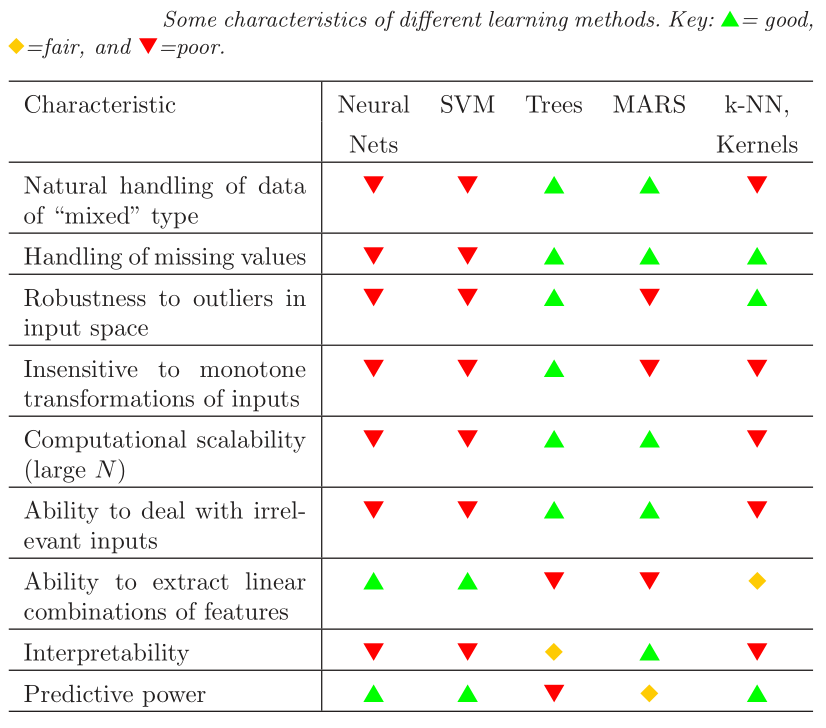
\includegraphics[scale=0.7]{method_comparison}
        \centering
        \caption {Comparison of Classifiers}
        \label{fig:classifier_comparison} %\ref{fig:classifier_comparison}
    \end{figure}


%%%%%%%%%%%%%%%%%%%%%%%%%%%%%%%%%%%%%%%%%%%%%%%%%%%%%%%%%%%%%%%%%%%%%%%%%%%
\section{Perpendicular distance in Maximum Margin Classifier}\label{sec:appendix_mmc_perpendicular_dist}
The equation of the plane is given by $\beta_{0} + \beta_{1}x_{1} + \cdots + \beta_{p}x_{p} = 0$. Let $x$ be the point whose perpendicular distance from the plane we want to calculate and let $x_{a}$ a point on the plane. The distance between $x$ and $x_{a}$ is
\begin{align*}
    d^{2} = \sum_{i=1}^{p} (x_{i} - x_{ai})^{2}
\end{align*}
and the minimum of this distance is the required perpendicular distance. Since $x_{a}$ lies on the plane, we have a constrained optimization
\begin{align*}
    \minimize_{x_{a1}, \ldots, x_{ap}} \sum_{i=1}^{p} (x_{i} - x_{ai})^{2} + \lambda (\beta_{0} + \beta_{1}x_{a1} + \cdots + \beta_{p}x_{ap})
\end{align*}

Taking the partial derivatives with respect to all components of $x_{a}$ and $\lambda$,
\begin{align*}
    -2(x_{i} - x_{ai}) + \lambda \beta_{i} &= 0 \quad \forall \quad i = 1, \ldots, p\\
    \beta_{0} + \beta_{1}x_{a1} + \cdots + \beta_{p}x_{ap} &= 0\\
    \implies \beta_{0} + \sum_{i=1} \beta_{i}(x_{i} - \frac{\lambda \beta_{i}}{2}) &= 0\\
    \implies 2\frac{\beta_{0} + \sum_{i=1}^{p} \beta_{i}x_{i}}{\sum_{i=1}^{p}\beta_{i}^{2}} &= \lambda\\
    \implies x_{i} - x_{ai} &= \beta_{i} \frac{\beta_{0} + \sum_{i=1}^{p} \beta_{i}x_{i}}{\sum_{i=1}^{p}\beta_{i}^{2}} \quad \forall \quad i = 1, \ldots, p\\
    \text{giving} \quad \sum_{i=1}^{p} \beta_{i}^{2} \frac{(\beta_{0} + \sum_{i=1}^{p} \beta_{i}x_{i})^{2}}{(\sum_{i=1}^{p}\beta_{i}^{2})^{2}} &= d^{2}\\
    \text{or} \quad \frac{(\beta_{0} + \sum_{i=1}^{p} \beta_{i}x_{i})^{2}}{\sum_{i=1}^{p}\beta_{i}^{2}} &= d^{2}
\end{align*}

Hence, the perpendicular distance is same as putting the point in the equation of the hyperplane and dividing by the norm of the coefficients. In the special case where the norm equals 1, the distance becomes $\lvert \beta_{0} + \sum_{i=1}^{p} \beta_{i}x_{i} \rvert$.


%%%%%%%%%%%%%%%%%%%%%%%%%%%%%%%%%%%%%%%%%%%%%%%%%%%%%%%%%%%%%%%%%%%%%%%%%%%
\subfile{appendix_lagrangian}

\end{document}